\documentclass[11pt]{article}
\usepackage{geometry,marginnote} % Pour passer au format A4
\geometry{hmargin=1cm, vmargin=1.5cm} % 

% Page et encodage
\usepackage[T1]{fontenc} % Use 8-bit encoding that has 256 glyphs
\usepackage[english,french]{babel} % Français et anglais
\usepackage[utf8]{inputenc} 

\usepackage{lmodern}
\usepackage[np]{numprint}
\setlength\parindent{0pt}

% Graphiques
\usepackage{graphicx,float,grffile}
\usepackage{tikz,pst-eucl,pst-plot,pstricks,pst-node,pstricks-add,pst-fun,pgfplots} 

% Maths et divers
\usepackage{amsmath,amsfonts,amssymb,amsthm,verbatim,scratch3}
\usepackage{multicol,enumitem,url,eurosym,gensymb,tabularx}

\DeclareUnicodeCharacter{20AC}{\euro}



% Sections
\usepackage{sectsty} % Allows customizing section commands
\allsectionsfont{\centering \normalfont\scshape}

% Tête et pied de page
\usepackage{fancyhdr} \pagestyle{fancy} \fancyhead{} \fancyfoot{}

%\fancyfoot[L]{Collège Faubert}
%\fancyfoot[C]{\thepage / 6}
%\fancyfoot[R]{Série Générale}

\renewcommand{\headrulewidth}{0pt} % Remove header underlines
%\renewcommand{\footrulewidth}{0pt} % Remove footer underlines

\newcommand{\horrule}[1]{\rule{\linewidth}{#1}} % Create horizontal rule command with 1 argument of height

\newcommand{\Pointilles}[1][3]{%
  \multido{}{#1}{\makebox[\linewidth]{\dotfill}\\[\parskip]
}}

\newtheorem{Definition}{Définition}

\usepackage{siunitx}
\sisetup{
    detect-all,
    output-decimal-marker={,},
    group-minimum-digits = 3,
    group-separator={~},
    number-unit-separator={~},
    inter-unit-product={~}
}

\setlength{\columnseprule}{1pt}


\begin{document}

\begin{center}
  \textit{Il faut apprendre, non pas pour l'amour de la connaissance, mais pour se défendre contre le mépris dans lequel le monde tient les ignorants.} - \textbf{Charlie Chaplin}
\end{center}

\begin{multicols}{2} 
\subsection*{Exercice 1} 

Peut-on construire un triangle à partir de ces trois longueurs ? 

\begin{itemize}[label={$\bullet$}]
  \item Triangle 1 : $12cm$ , $13cm$  et $21cm$.
  \item Triangle 2 : $54cm$ , $25cm$ et $12cm$.
  \item Triangle 3 : $16cm$ , $24cm$ et $16cm$.
\end{itemize} \columnbreak

\subsection*{Exercice 2} 

\begin{itemize}[label={$\bullet$}]
  \item $AB = 10cm$ et $BC = 13cm$. \\ Quelles sont les longueurs possibles pour AC ?
  \item $NO = 123cm$ et $MO = 251cm$. \\ Quelles sont les longueurs possibles pour MN ?
  \item $XZ = 24,6cm$ et $XY = 31,8cm$. \\ Quelles sont les longueurs possibles pour YZ ?
\end{itemize}
\end{multicols}

\subsection*{Exercice 3} 

Tracer un triangle ABC tel que : $AB = 6,4cm$ , $AC = 5,2cm$ et $BC = 7,5cm$. 

\subsection*{pb1 : Réalisation d'un covering sur une Lamborghini} 

  \textit{Le covering est une spécialité de préparation automobile visant à appliquer un film de décoration ou de protection sur l'ensemble d'une voiture.} 

  Un carrossier spécialiste en covering facture l'opération 4\,200€ pour une Lamborghini. Le client souhaite un covering de décoration DBZ.
  Pour réaliser ce covering, le carrossier doit acheter le film de décoration 2\,800€. Il compte 6h pour poser le film de décoration correctement. 

  Quel est son bénéfice ? 


\subsection*{pb2 : Entretien des roues et du freinage sur une Porsche} 

  Lewis Hamilton souhaite faire du circuit avec sa Porsche 911. Mais avant d'enchaîner les tours de piste, il souhaite changer les 4 pneus ainsi que les 4 plaquettes de frein. 

  Il hésite entre deux offres : 

  \begin{itemize}[label={$\bullet$}]
    \item Norauto : 1 roue et 1 plaquette neuves pour 64€ les deux.
    \item Midas : 2 roues neuves pour 75€ et 2 plaquettes pour 56€. 
  \end{itemize} 

Quelle est l'offre la plus avantageuse ?

\subsection*{pb3 : Pit Stop F1} 

  Dans une course de Formule 1, 22 mécaniciens vont en même temps s'occuper de changer les roues, mettre du carburant et réaliser diverses petites actions importantes. Les meilleurs équipes arrivent à changer les 4 pneus autour des 2,2 secondes. 

  L'équipe Red Bull réalise un excellent temps de 2 secondes pour le Pit Stop. Cela permet au pilote Max Verstappen de gagner la course et de monter sur la première marche du podium. Il gagne une prime de 67\,000€. Il garde 12\,000€ pour lui et souhaite que l'équipe de mécaniciens se partage équitablement le reste. 

Quelle somme d'argent va recevoir chaque mécanicien de l'équipe Red Bull ?

\begin{multicols}{3} 
 \begin{figure}[H]
    \centering
    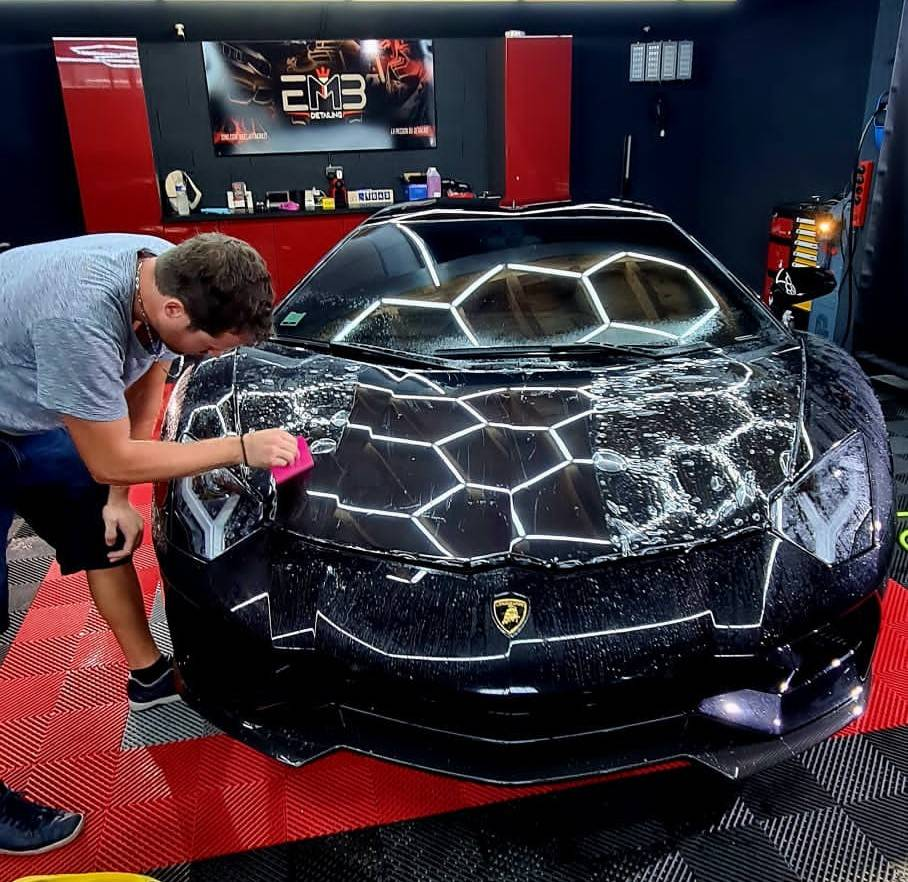
\includegraphics[width=0.8\linewidth]{5x2-inegalite-triangulaire/lambo.jpg}
  \end{figure}

  \begin{figure}[H]
    \centering
    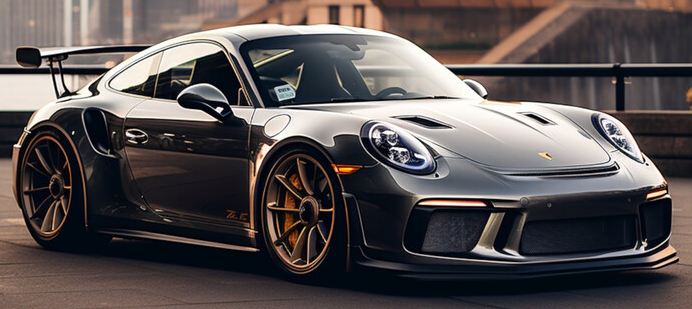
\includegraphics[width=\linewidth]{5x2-inegalite-triangulaire/porsche.png}
  \end{figure} 

    \begin{figure}[H]
    \centering
    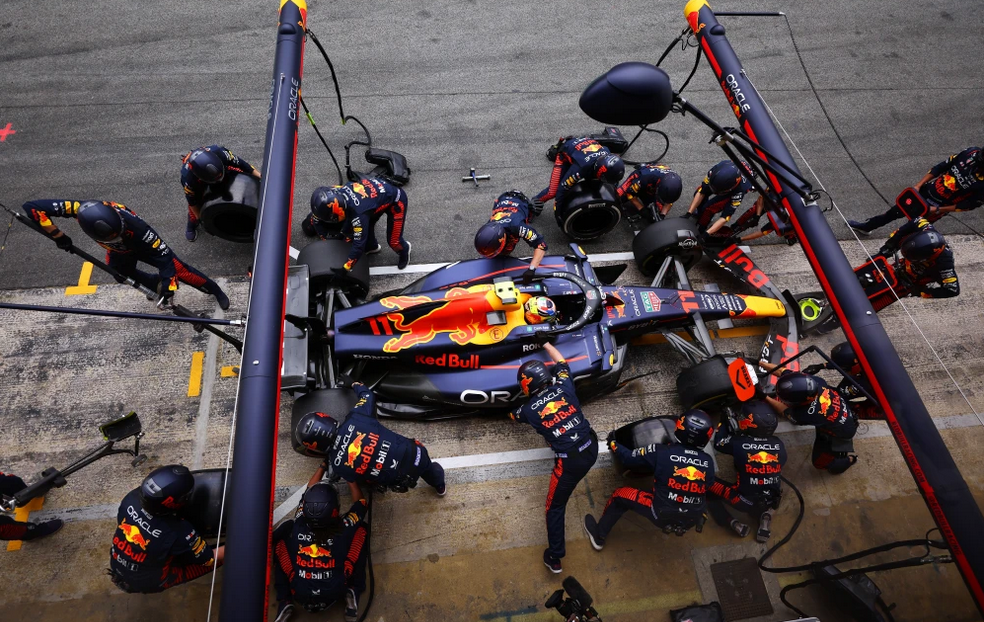
\includegraphics[width=\linewidth]{5x2-inegalite-triangulaire/f1.png}
  \end{figure} 
\end{multicols}

\end{document}